\section{Material e Métodos}

% Na Figura \ref{fig:diag}, são mostradas as etapas realizadas no estudo, que incluem a coleta das amostras, aquisição das imagens, obtenção dos valores de referência, pré-processamento, construção e validação dos modelos e a análise estatística. Na seção seguinte todas as etapas serão descritas.

% \begin{figure}[H]
% \centering
%     \caption{Etapas realizadas no estudo.}\label{fig:diag}
%     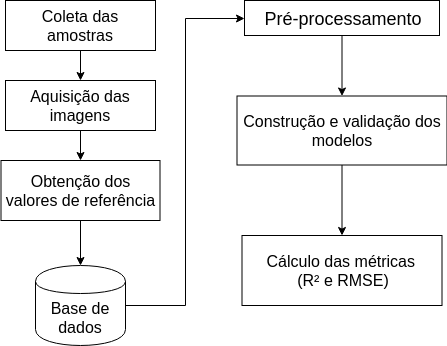
\includegraphics[scale=0.5]{imgs/exp_artigo.png}
% \end{figure}

\subsection{Amostras}

Foram utilizadas mangas cv. ‘Palmer’ coletadas manualmente em pomar comercial da Fazenda Special Fruit Importação e Exportação Ltda., localizada no município de Petrolina–Pernambuco, região de clima do tipo BSwh (semiárido, tipo estepe, muito quente, com estação chuvosa no verão), segundo classificação de Koppen, que fica a 9º18'13,5''S e 40º40'04,7''O, com altitude de aproximadamente 380 m.

A Fazenda tem 114 hectares plantados com manga ‘Palmer’. O lote em estudo tem 3,47 há, com espaçamento da cultura de 6 X 4 m e é utilizado o sistema de irrigação de microaspersão, com turno de rega diário e com lâmina ajustada ao longo do ciclo. As mangueiras receberam todos os tratos culturais de acordo com as exigências da cultura.

Foram selecionadas trinta plantas, distribuídas em cinco fileiras de plantio de um lote do pomar. Foram coletados 600 frutos no total, oitenta em cada fase: 35, 50, 65, 80, 95, 110, 125, 140, 165 e 180 dias após a floração (DAF), ponto de colheita comercial adotado pela Fazenda. A colheita foi realizada no período da manhã, utilizando-se uma tesoura de poda para o corte do pedúnculo.

Após a coleta, os frutos foram transportados cuidadosamente até o Laboratório de Armazenamento de Produtos Agrícolas (LAPA) da Universidade Federal do Vale do São Francisco, campus Juazeiro-BA, onde foram lavados em água corrente, um a um, e imersos em solução de 150 mg de cloro por litro de água por 15 minutos, com posterior enxague para remoção do excesso de cloro e secagem em temperatura ambiente. Em seguida, foi determinada a massa dos frutos com auxílio de balança semi-analítica com precisão de 0.01 g.

A firmeza do fruto foi determinada com o auxílio de um penetrômetro digital modelo PTR 300, com ponteira de 6 mm de diâmetro. Foi realizada uma leitura por fruto, na porção equatorial, e o resultado foi expresso em Newtons (N). Os sólidos solúveis totais (SST) foram determinados de forma destrutiva em filtrado da polpa centrifugada, utilizando um refratômetro digital (Hanna – HI 96804), sendo os resultados expressos em ºBrix (AOAC, 1997). Por fim, a acidez titulável foi determinada através de titulação com solução de hidróxido de sódio (0.1 M NaOH) com 1\% de fenolftaleína como indicador, também de acordo com a metodologia da AOAC (1997). 

Os valores de referência supracitados foram determinados após o processo de aquisição das imagens, realizada em parceria com o Laboratório de Energia na Agricultura (LENA) da mesma Universidade. O sistema de aquisição de imagens de reflectância foi constituído por uma câmera fotográfica Canon T5i, caixa de interior preto fosco, fonte de alimentação ajustável e uma caixa de controle de acendimento de LEDs, representado na Figura \ref{fig:caixa} O sistema de iluminação era constituído por 3 LEDs Solderless XPE2 de 3W da CREE, branco frio 5000K a 8300K, dispostos a uma distância angular de 120º entre eles. 

\begin{figure}[!htb]
\centering
    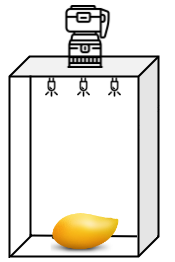
\includegraphics[scale=0.7]{imgs/mangobox.png}
    \caption{Esquema de aquisição das imagens.}\label{fig:caixa}
\end{figure}

Para o processo de aquisição das imagens foi obtida uma imagem para cada lado de cada fruto (considerando a posição de repouso), através da câmera ajustada com foco manual, ISO-100; tempo de exposição 1/2s; F/5.6; distância focal de 48mm.

\subsection{Pré-processamento}
Como as imagens obtidas possuíam ruído e informações irrelevantes, foi necessário realizar o pré-processamento das mesmas. Foram testadas diferentes configurações de algoritmos, de forma a remover a maior quantidade possível de ruído sem perda de informações relevantes da imagem. Apesar das fotos terem sido tiradas em um ambiente controlado, as imagens resultantes variaram quanto ao ruído nelas contido, devido ao acúmulo de sujeira na câmara com o passar das semanas do experimento. Sendo assim, as configurações das técnicas variaram para cada imagem.

A primeira técnica aplicada foi o filtro da mediana, visando a remoção de manchas contidas nas imagens. O tamanho de janela que garantiu uma melhor remoção de ruído na maioria das imagens foi de 11x11 pixels. Após isso, as imagens foram segmentadas através do algoritmo de Otsu, de forma que as mangas fossem isoladas do fundo. Com isso, notou-se nas imagens a presença de pequenos pontos que não foram removidos pelo filtro da mediana. Apesar de a remoção dos mesmos ter sido possível com uma segunda filtragem pela mediana, notou-se uma perda de detalhes na manga. Sendo assim, optou-se por empregar a operação de abertura, operação morfólogica através da qual pequenos pontos de uma imagem podem ser removidos. 

A utilização destas técnicas não garantiu uma remoção completa das sombras contidas na imagem. Assim, utilizou-se a limiarização simples para este fim, visto que a intensidade dos pixels correspondentes às sombras era, em geral, visivelmente menor que a intensidade dos pixels das mangas. Como a limiarização simples resultou na remoção de partes da manga, além das sombras delas, empregou-se a operação morfológica de fechamento para o preenchimento das mangas.

Por fim, foram traçados os contornos das mangas, visando a remoção de partes da imagem que não continham a fruta. A Figura \ref{fig:prep} mostra uma imagem original e pré-processada.

\begin{figure}[H]
\centering
    \subcaptionbox{}{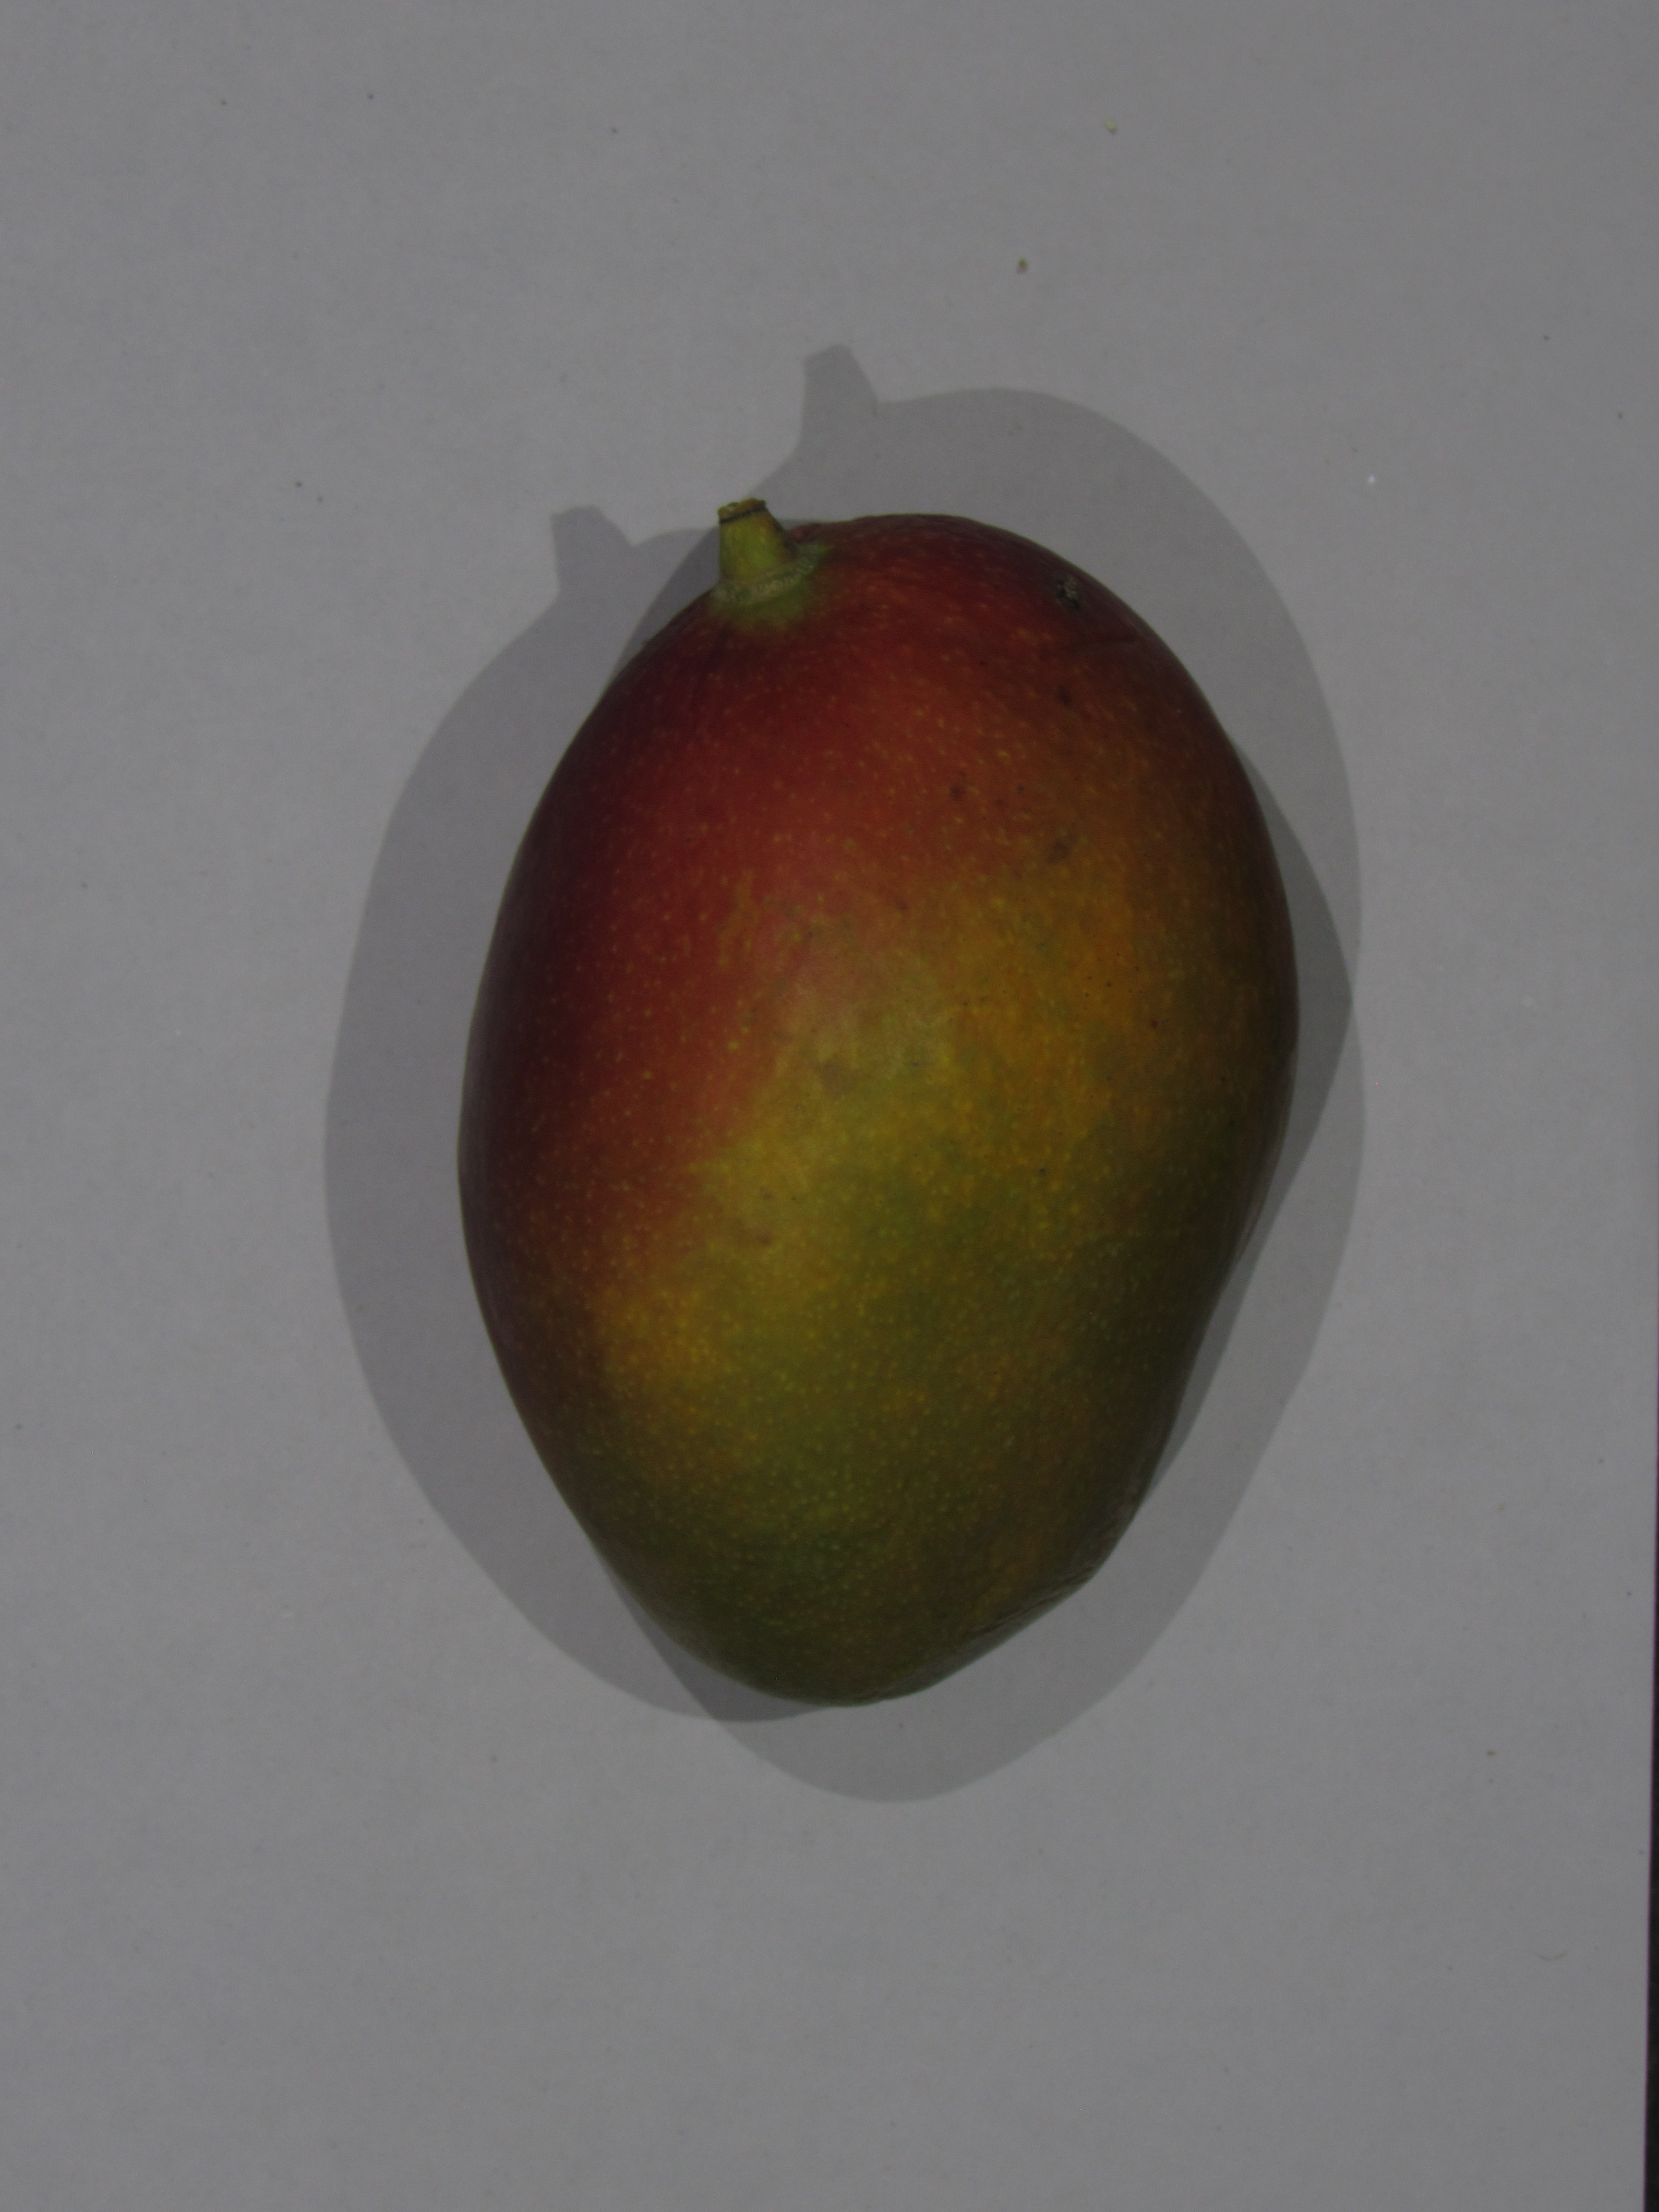
\includegraphics[scale=0.035]{imgs/sem_processamento.JPG}}
    \subcaptionbox{}{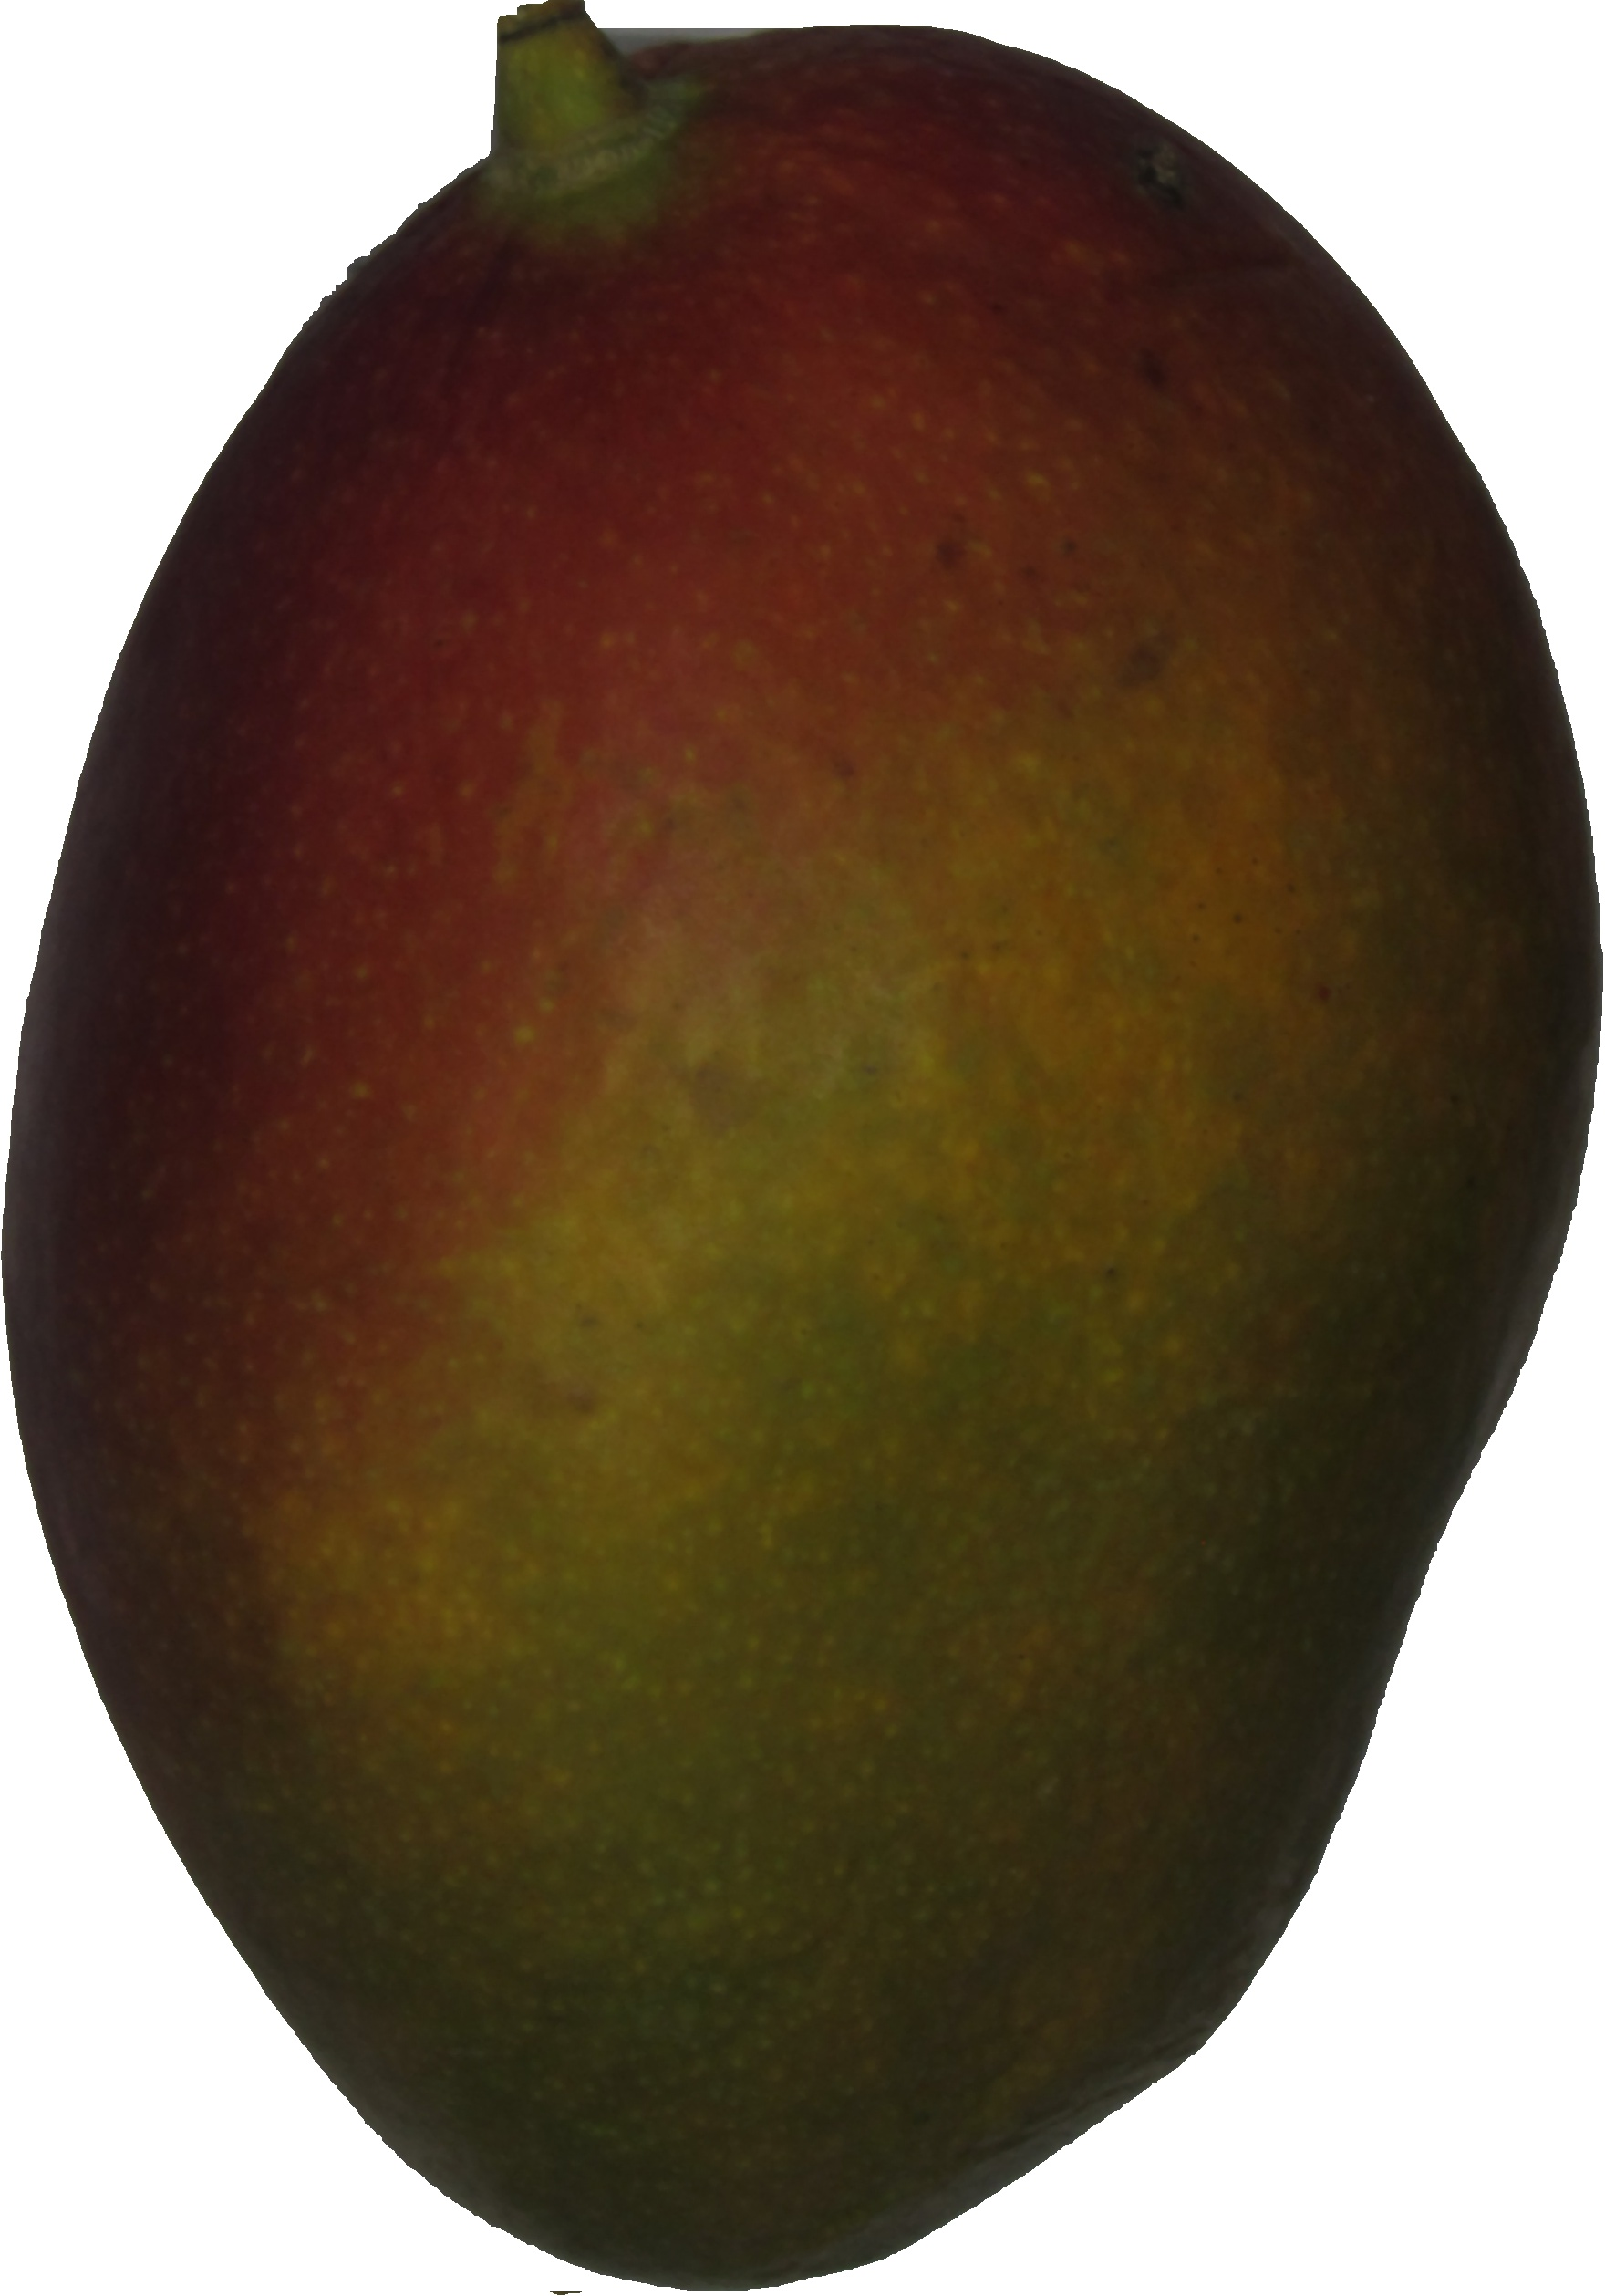
\includegraphics[scale=0.062]{imgs/processada.JPG}}
    \caption{Efeito do pré-processamento. (a) Imagem original (b) Imagem pré-processada.}\label{fig:prep}
\end{figure}

Posteriormente, as variáveis mencionadas na Tabela \ref{tbl:var} foram extraídas para cada imagem. Todos os algoritmos de pré-processamento de imagens, assim como a extração de variáveis, foram realizados através da linguagem de programação Python (versão 3.6.7), com o auxílio da biblioteca OpenCV (versão 3.4.4).

\subsection{Método e métricas de avaliação de desempenho}
Antes da construção dos modelos foi realizada uma reamostragem das imagens, devido ao desbalanceamento presente na base de dados. Como havia 600 imagens de mangas tiradas antes da colheita e apenas 240 imagens tiradas após ela, foi feita uma repetição aleatória das imagens deste período até que fosse obtida uma quantidade igual de imagens nos dois períodos.

% Assim, foram treinadas \textit{Random Forests} para cada subconjunto de variáveis definido na Tabela \ref{tbl:var}, além do subconjunto que reúne todas as variáveis, para a determinação da idade das mangas, sua massa, SST, firmeza e acidez titulável. Além disso, também foram construídos modelos com Regressão linear, para comparação direta com os melhores modelos da literatura.

Para a avaliação da capacidade preditiva dos modelos, foi utilizada a estratégia de validação cruzada 5-\textit{fold} (5-\textit{fold cross validation}). Ela é empregada para assegurar a robustez do modelo, através da divisão do conjunto de dados em 5 subconjuntos disjuntos, com uma alocação das amostras para o conjunto de treinamento ou teste (Zhang & Yang, 2015). Assim, um dos subconjuntos foi utilizado como teste e os 4 demais para o treinamento, de forma que o modelo realizasse a predição para dados desconhecidos. Este procedimento foi repetido 5 vezes, alterando os subconjuntos a cada vez.

As predições resultantes foram avaliadas através de métricas, tais como o coeficiente de correlação e raiz do erro quadrático médio (RMSE), empregadas nos artigos em que a regressão foi realizada. Estes indicadores medem, respectivamente, o grau de dependência entre as variáveis de entrada e saída e a magnitude média dos erros estimados (Alves; Vecchia, 2011), conforme as equações abaixo:

\begin{equation} \label{eq:r}
	R = \frac{\sum_{i=1}^n (x_i - \overline{x})(y_i - \overline{y})}{\sqrt{\sum_{i=1}^n(x_i - \overline{x})^2} \sqrt{\sum_{i=1}^n (y_i - \overline{y})^2}}
\end{equation}

\begin{equation} \label{eq:rmse}
	RMSE = \sqrt{\frac{1}{n} \sum_{i=1}^n (y_i - \hat{y}_i)^2}
\end{equation}

Em que $x_i$ é o valor da variável de entrada, $\overline{x}$ é a média dos valores de $x$, $y_i$ é o valor real da variável de saída, $\overline{y}$ é a média dos valores de $y$, $n$ é o número de amostras e $\hat{y}_i$ é o valor previsto para a variável de saída.

\subsection{Abordagem comparada}

Na Tabela \ref{tbl:artigos_var}, são mostradas as variáveis de entrada utilizadas na literatura para predição de massa, SST, firmeza ou acidez titulável, assim como a técnica de inferência utilizada. Nota-se que para todos os trabalhos foi utilizada a Regressão linear para predição do atributo alvo. Entretanto, esta técnica assume um relacionamento linear entre as variáveis de entrada e de saída, o que, apesar de ter fornecido bons resultados para as variedades empregadas pelos autores, pode não ser o caso para a 'Palmer'.

Na predição de cada um dos atributos de qualidade, foi comparada a abordagem empregada na literatura e o melhor subconjunto obtido pela \textit{Random Forest}. As mesmas variáveis utilizadas pelos autores serão utilizadas como entrada em uma Regressão linear e os resultados obtidos serão comparados diretamente aos resultados obtidos pelo melhor modelo \textit{Random Forest}.

\begin{table}[H]
\centering
\caption{Atributo de qualidade, variáveis de entrada e técnica de inferência empregadas na literatura.}\label{tbl:artigos_var}
\begin{tabular}{lll}
\hline
Atributo de qualidade & Variáveis de entrada  & Técnica de inferência \\ \hline
Massa   & Número e pixels & Regressão linear\\ \hline
SST     & Valor médio da matiz & Regressão linear\\ \hline
Firmeza & Valor médio de L* & Regressão linear \\ \hline
acidez titulável  & Valor médio de L* & Regressão linear \\
\hline
\end{tabular}
\end{table}

A partir da comparação dos resultados, será possível determinar a melhor abordagem para predição de atributos de qualidade em mangas 'Palmer'. 

\subsection{Análise estatística}
\label{S:1}
